\newcommand{\chapterpepperusecase}{Kapitel 6. }

\chapter{Implementierung der Anwendungsfälle}
\label{sec:Pepper_Anwendungsfälle}
\lhead{\chapterpepperusecase \emph{Pepper - Anwendungsfälle}}

Im Folgenden werden wir auf die Implementierung unserer Anwendungsfälle eingehen. Hierbei gehen wir zuerst auf die Planung und anschließend auf die Bereitstellung der Daten in unserem Server und in externe Scripts ein. Anschließend erläutern wir die Implementation und Weiterverarbeitung der einzelnen Anwendungsfälle in Android Studio.

\section{Mensa}

Der Anwendungsfall für die Mensa ist in zwei Teile aufgeteilt. Der erste Teil ist das Anzeigen des Mensaplans auf dem Tablet von Pepper. Sollte der User explizit nach dem Mensaplan fragen, soll Pepper eine Übersicht des Mensaplans der aktuellen Woche anzeigen. 
Der zweite Teil ist das verbale Beschreiben des Mensaangebots. Hierbei soll Pepper für jeden Wochentag erzählen können, welche Angebote in der Mensa zurzeit zur Verfügung stehen. Die Mensa der Hochschule Bremerhaven bietet jeden Wochentag immer zwei Angebote an. Das zweite Angebot ist dabei immer vegetarisch. Pepper muss dementsprechend in der Lage sein, beide Angebote beschreiben zu können. 

Um die verschiedenen Daten über die Mensa Angebote abrufen zu können, verwenden wir unseren Server, der diese Daten bereitstellt. Der Server bekommt diese Daten aus einem externen Python Script.

\subsection{Script um Mensadaten aufzurufen}

Um die Daten auf dem Server anzeigen zu lassen, wird ein Python script verwendet, dass sich diese Daten aus der offiziellen Hochschule Bremerhaven Mensa Webseite zieht. 

Webseite: \url{https://www.stw-bremen.de/de/cafeteria/bremerhaven}

Auf dieser Webseite befinden sich die aktuellen Angebote für die nächsten fünf Tage in einer Tabelle und den aktuellen- sowie nächsten Wochenplan als PDF-Format. Mit dem Python Script werden die einzelnen Daten aus der Webseite gezogen und als JSON String umgewandelt. Das ziehen der Daten aus der Webseite wird mithilfe des Framework ``BeautifulSoup'' durchgeführt, dass erlaubt, XML- und HTML-Dokumente zu ``parsen''.

\begin{lstlisting}
menulist = soup.select("tbody")

menu = {}
day = ["Montag","Dienstag", "Mittwoch", "Donnerstag", "Freitag"]
offer1 = []
offer2 = []
\end{lstlisting}

Die Mensa Angebote befinden sich auf der Webseite in einer Tabelle, weswegen wir auf alle ``tbody''-Elemente mit der Funktion ``soup.select'' zugreifen. Diese werden als Array in die Variable ``menulist'' initialisiert. Anschließend werden die Variablen deklariert, aus denen später der JSON string entstehen soll. 

\begin{lstlisting}
for i in range(10):
    tmp = (str(menulist[i]).split('description">',1)[1]).rsplit
    ("</td><td",2)[0]
    tmp = tmp.replace("\n","").replace("\r","").replace("a1","")
    .replace("amp;","")
    tmp = re.sub('<sup>.*?</sup>', '', tmp)
    if(i%2==0):
        offer1.append(tmp)
    else:
        offer2.append(tmp)
    menu["day"] = day
    menu["offer1"] = offer1
    menu["offer2"] = offer2

with open(folder_location+"mensadata.json", "w+") as f:
    json.dump(menu, f, ensure_ascii=False)
\end{lstlisting}

Da sich die Daten in den ``tbody''-Elementen schwer lesen lassen, werden diese mit mehreren ``split'' und ``replace'' Funktionen in lesbare Mensa Angebote umgeformt und in den einzelnen Variablen eingefügt. Die If-Bedingung wird verwendet, um das erste- und zweite Angebot voneinander zu trennen. Anschließend wird das ``menu'' Objekt mit den keys ``day'', ``offer1'' und ``offer2'' und den values der jeweiligen Arrays initialisiert.
Zum Schluss wird das ``menu'' Objekt in JSON mit der ``json.dump'' Funktion umgewandelt.

Um den aktuellen Wochenplan im Script herunterzuladen und weiterzuverarbeiten, wird die Programmbibliothek Poppler vorausgesetzt. Poppler wird in Unix-ähnlichen Betriebssystemen dazu verwendet, PDF-Dateien anzuzeigen.

\begin{lstlisting}
response = requests.get(url)
soup= BeautifulSoup(response.text, "html.parser")
menucard = ((str(soup.select("a[href$='/print']")[0])
.rsplit(' target',1)[0]).split("href=",1)[1])
.replace('"','')
urllib.request.urlretrieve(menucard, folder_location+"Mensaplan.pdf")
\end{lstlisting}

Mit den ersten beiden Zeilen Code wird der komplette HTML-Inhalt der Webseite in die Variable soup initialisiert. Da wir die URL des aktuellen Wochenplans benötigen, muss dieser aus dem HTML Code gezogen werden. Der Standort dieser URL ist im HTML Code fest verankert, weswegen wir mithilfe von soup.select, die URL herausfiltern und mit mehreren ``split'' und ``replace'' Funktionen zu einer gültigen URL umformen können. Dieser Zwischenschritt ist nötig, da sich die URL jede Woche ändert. Anschließend wird die URL aufgerufen und als ``Mensaplan.pdf'' abgespeichert.

\begin{lstlisting}
img = convert_from_path(folder_location+"Mensaplan.pdf", 500)[0]

area = (0, 200, 4134, 2800) # R T L B
cropped_img = img.crop(area)

area = (0, 5200, 4134, 5800)
cropped_img2 = img.crop(area)
mergeImgs([cropped_img, cropped_img2])
.save(folder_location+'images/mensaplan.png', 'JPEG')
\end{lstlisting}

Anschließend wird mit der Funktion ``convert\_from\_path'' das PDF in ein Bildformat konvertiert und in die Variable ``img'' installiert. Hierfür wird das Framework ``pdf2image'' verwendet, das vorab mit ``pip'' installiert werden muss. 

Nun ist das Bild jedoch im Hochformat und kann sehr schlecht auf dem Tablet von Pepper angezeigt werden. \ref{fig:Mensaplan} Somit haben wir das Bild in zwei Teile geschnitten und im Querformat zusammengefügt. Um das Bild zu schneiden, haben wir das Framework PIL verwendet. Nun kann genau angegeben werden, wie das Bild geschnitten werden soll. In der Variable ``area'' haben wir jeweils immer vordefiniert, wie weit das Bild in welcher Richtung ausgeschnitten werden soll. Die Reihenfolge der Richtungen lautet wie folgt: 
(Rechts Oben Links Unten) (0, 200, 4134, 2800)

Zuerst haben wir den oberen Teil des Mensaplans ausgeschnitten, der die einzelnen Angebote enthält und anschließend die Legende, die sich im unteren Bereich der PDF befindet. 

Nun müssen beide Bilder zusammengefügt werden. Dies wurde in der Methode ``mergeImgs'' durchgeführt.


\begin{lstlisting}
def mergeImgs(imgs):
    min_img_width = min(i.width for i in imgs)
    
    total_height = 0
    for i, img in enumerate(imgs):
    
    if(img.width > min_img_width):
        imgs[i] = img.resize((min_img_width, int(img.height / 
        img.width * min_img_width)), Image.ANTIALIAS)
    total_height += imgs[i].height
    
    img_merge = Image.new(imgs[0].mode, (min_img_width, total_height))
    y = 0
    for img in imgs:
        img_merge.paste(img, (0, y))
    
        y += img.height
    return img_merge
\end{lstlisting}

In dieser Funktion wird zuerst die Breite und Höhe des neu zusammengefügten Bildes ermittelt. Sollten die beiden Bilder eine unterschiedliche Breite besitzen, wird das breiteste Bild verkleinert. Dies geschieht in der For-Schleife, wo jedes einzelne Bild überprüft wird. 
Anschließend wir ein neues ``img\_merge'' Objekt erzeugt, das mit der minimalsten Breite und addierten Höhe der beiden Bilder initialisiert wird. Zum Schluss werden die beiden Bilder in das Objekt eingefügt und heruntergeladen.

\begin{figure}[H]
    \centering
    \includegraphics[width=15cm]{Figures/AppChapter/mensa_3.png}
    \caption{Mensaplan - cropped}
    \label{fig:Mensaplan}
    \centering
\end{figure}

\subsection{Weiterleitung zum NodeJS Server}

\ref{fig:cron} Das Script befindet sich auf dem Hopper und wird mit crontab jeden Montag einmal ausgeführt. Es ist wichtig, dass das Script nur jeden Montag ausgeführt wird, da die Mensa Angebote nur für die nächsten fünf Tage zur Verfügung kann. Sollte das Script zum Beispiel an einem Mittwoch ausgeführt werden, so würden die Tage Montag und Dienstag fehlen.

\begin{figure}[H]
    \centering
    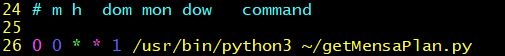
\includegraphics[width=13cm]{Figures/AppChapter/mensa_4.JPG}
    \caption{getMensaPlan - Crontab}
    \label{fig:cron}
    \centering
\end{figure}

Das erzeugte JSON Objekt und das zugeschnittene Bild des Mensaplans werden anschließend in den public static Ordner vom Node Server eingefügt.

\subsection{Bereitstellen der Mensadaten auf dem Server}

Mit dem folgenden Code werden die Daten aus den jeweiligen “/static” Ordnern an die Webseite gesendet:

\begin{lstlisting}
router.get('/docker-hbv-kms-http/api/v1/mensadata', (req, res) => {
    const filePath = `${__dirname}/../static/data/mensadata.json`;
    const jsonData = JSON.parse(fs.readFileSync(filePath, 'latin1'));
    res.send(jsonData);
});

router.get('/docker-hbv-kms-http/api/v1/mensadata/img', (req, res) => {
    const filePath = `${__dirname}/../static/images/mensaplan.png`;
    const img = fs.readFileSync(filePath);
    res.writeHead(200, {
        'Content-Type': 'image/png'
    });
    res.end(img, 'binary');
});    
\end{lstlisting}

\ref{fig:mensaapi} In folgendem Pfad befindet sich nun unser JSON Objekt, mit allen Mensaangeboten der aktuellen Woche.\\
\url{https://informatik.hs-bremerhaven.de/docker-hbv-kms-http/api/v1/mensadata}

\begin{figure}[H]
    \centering
    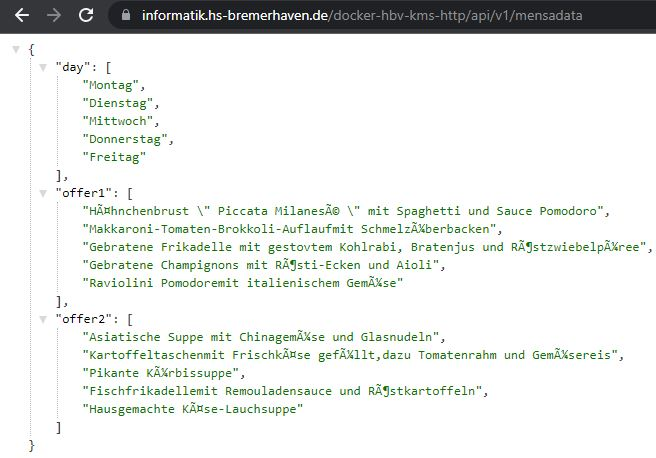
\includegraphics[width=13cm]{Figures/AppChapter/mensa_5.JPG}
    \caption{Mensadaten - API}
    \label{fig:mensaapi}
    \centering
\end{figure}

Der aktuelle Wochenplan ist in png-Format unter folgendem Link erreichbar:\\
\url{https://informatik.hs-bremerhaven.de/docker-hbv-kms-http/api/v1/mensadata/img}


\subsection{Anzeigen der Mensadaten in Android Studio}

Wie bereits erwähnt, soll Pepper mithilfe von Sprache in der Lage sein, den Mensaplan auf sein Tablet anzuzeigen und Informationen 
über die verschiedenen Angebote jedes Wochentags zu geben. Um sich den Mensaplan anzeigen zu lassen, haben wir zuerst ein neues 
Gesprächsthema in unserem Haupt-Topic erstellt. 

\begin{lstlisting}
u:(["Ich hab{e} hunger" "Zeig {mir} {den} Mensaplan"] ) 
^execute(VariableExecutor, qiVariableMensa, Plan) Hier hast du eine 
Uebersicht ueber den Mensaplan

case("qiVariableMensa"):
String day = params.get(1);
if(day.equals("Plan")){
    ...
}
\end{lstlisting}

Sobald der User nach dem Mensaplan fragt, wird die ``runWith'' Methode mit den Parametern ``qiVariableMensa'' 
und ''Plan'' in der ``VariableExecutor'' Klasse aufgerufen. In dieser Methode wird anschließend nach dem switch 
case ``qiVariableMensa'' gesucht. Da wir einen zweiten Mensaanwendungsfall besitzen, müssen wir diese beiden Fälle 
voneinander unterscheiden können. Aus diesem Grund wurde ein weiterer String Parameter mit dem Namen ``Plan'' mitgegeben, 
um über einer If-Bedingung diese beiden Fälle zu trennen. 
Nun gibt es mehrere Möglichkeiten, das Bild aus dem Server zu nehmen und auf dem Tablet von Pepper anzeigen zu lassen. Die 
einfachste Methode wäre über den WebViewer. Hierfür hätten wir lediglich die URL benötigt, um die Webseite mit dem Bild auf dem 
Tablet anzeigen zu lassen. Die Bildgröße des Mensaplans besaß jedoch eine viel zu große Auflösung (3200 x 4134 px), sodass nur ein 
Teil des Bildes auf dem Tablet angezeigt werden konnte.
Auf dem Node Server oder in Android Studio könnte die Auflösung theoretisch manuell umgestellt werden können, jedoch haben wir uns 
für einen anderen Weg entschieden. 

Wir haben uns anschließend dazu entschieden, das Bild in Android Studio als Bitmap vom Node Server herunterzuladen. Eine Bitmap 
ist eine Zahlenmatrix von einem Bild, wo jeder Pixel die jeweiligen Farbinformationen enthält.


\begin{lstlisting}
String url_str = "https://informatik.hs-bremerhaven.de/
docker-hbv-kms-http/api/v1/mensadata/img";
InputStream srt = new URL(url_str).openStream();
final Bitmap bitmap = BitmapFactory.decodeStream(srt);
    
ma.runOnUiThread(() -> {
    ma.setContentView(R.layout.mensa_layout);
    ImageView imageView = (ImageView) ma.findViewById(R.id.iMensa);
    imageView.setImageBitmap(bitmap);
});
\end{lstlisting}

In diesem Code wird das Bild in einen InputStream initialisiert. Ein InputStream ist eine Folge von Bytes, womit sich Daten lesen 
lassen können. Der InputStream wird mithilfe der ``BitmapFactory.decodeStream'' Funktion in eine Bitmap umgewandelt. 
Anschließend kann eine Imageview mittels der Id mit der Bitmap initialisiert werden. 

Nun kann Pepper auf die Frage ``Zeig mir den Mensaplan'' ein Bild von dem aktuellen Mensaplan auf sein Tablet zeigen. 

\begin{figure}[H]
    \centering
    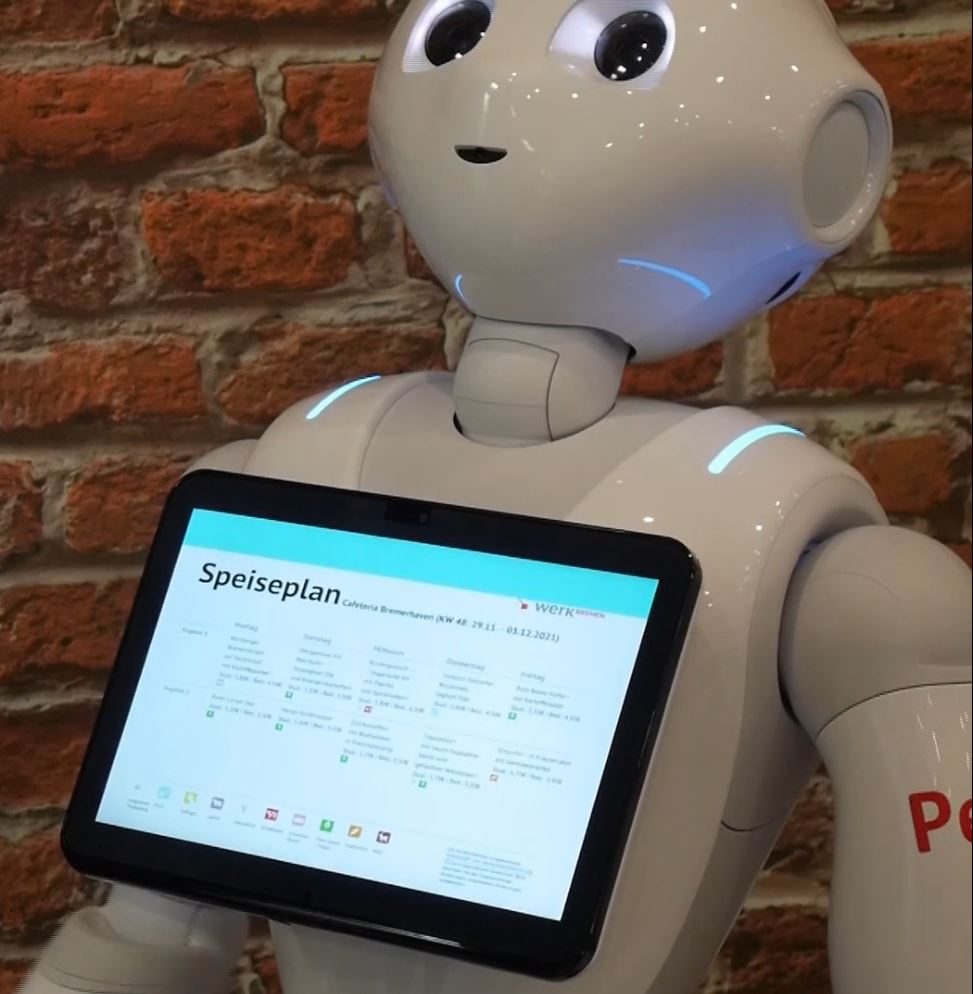
\includegraphics[width=6cm]{Figures/AppChapter/rx2.JPG}
    \caption{Mensaplan auf Hopper}
    \label{fig:mensaplanPepper}
    \centering
\end{figure}

Als Nächstes wird ein weiteres Gesprächsthema erstellt, dass Pepper erlaubt, auch verbal Informationen über die Mensa Angebote zu geben.

\begin{lstlisting}
concept:(week) [Montag Dienstag Mittwoch Donnerstag 
Freitag Heute Morgen Uebermorgen]

u:({was} {gibt{s}} {es} {zu} essen {am} _[~week]) $day=$1 
^execute(VariableExecutor, qiVariableMensa, $day) $day gibt 
es entweder $qiVariableMensa

u:({was} {gibt{s}} {es} {am} _[~week] {zu} essen) $day=$1 
^execute(VariableExecutor, qiVariableMensa, $day) $day gibt 
es entweder $qiVariableMensa
\end{lstlisting}

Hier wird die Variable ``\$day'' mit dem Wochentag in  ``\_[~week]'' initialisiert, dass in der Frage genannt wurde. Wenn der User 
zum Beispiel fragt: ``Was gibt es am Mittwoch zu essen'', wird Mittwoch in die Variable ``\$day'' initialisiert. In dem Konzept 
wurden nicht nur Wochentage, sonder auch Wörter wie Heute, Morgen und Übermorgen hinzugefügt. Somit kann der User auch fragen, was es zum Beispiel 
morgen zu essen gibt. 
Anschließend wird wieder die ``runWith'' Methode aufgerufen mit den Parameter ``qiVariableMensa'' und dem Wochentag, der genannt wurde.
In der VariableExecutor Klasse wird nun die Antwort vorbereitet, die Pepper zu der Frage geben soll. Hierfür wird die ``getOffer'' Methode in 
der HelperCollection Klasse aufgerufen.

\begin{lstlisting}
HttpURLConnection con = getConnection("https://informatik.
hs-bremerhaven.de/docker-hbv-kms-http/api/v1mensadata");

BufferedReader in = new BufferedReader(new InputStreamReader(
    con.getInputStream()));
String inputLine;
StringBuffer response = new StringBuffer();
while ((inputLine = in.readLine()) != null) { 
    response.append(inputLine); 
}
in.close();

JSONObject myResponse = new JSONObject(response.toString());
String tmp = myResponse.getString("offer1");
String [] offer1 = tmp.split("\",\"", -1);
tmp = myResponse.getString("offer2");
String [] offer2 = tmp.split("\",\"", -1); 
\end{lstlisting}

Zuerst werden die Daten aus dem Server aufgerufen und mithilfe des BufferedReader in das StringBuffer Objekt response initialisiert. 
Anschließend wird ein JSON Objekt aus dem response erstellt. Für uns war es leichter, die Daten in einem Array zu speichern, weswegen 
wir zwei String Arrays mit den jeweiligen Mensa Angeboten initialisiert haben.

\begin{lstlisting}
Calendar calendar = Calendar.getInstance();
int curday = calendar.get(Calendar.DAY_OF_WEEK) - 2;    
\end{lstlisting}

Nun wird mit der Calendar Bibliothek von Java, der aktuelle Wochentag ermittelt und als Zahl in curday gespeichert. 
Wäre der aktuelle Wochentag ein Montag, so würde curday mit einer 0 initialisiert. Sollte es ein Mittwoch sein, dann wäre curday eine 
2 usw. 
Somit können wir die ``offer1'' und ``offer2'' Arrays mit dem genauen Index des aktuellen Wochentags ermitteln.

\begin{lstlisting}
String [] daylist = {"Montag","Dienstag","Mittwoch","Donnerstag",
                    "Freitag"};
String [] spcdays = {"Heute", "Morgen", "Uebermorgen"};
String answer = "";

for(int i = 0; i < spcdays.length; ++i){
if(day.equals(spcdays[i])){
        if((curday + i) > 5){
            answer ="Am Wochenende ist die Mensa leider geschlossen";
            break;
        }
        answer = offer1[curday + i].replaceAll("\"", "").replace(
            "[","").replace("]","");
        answer += " oder " + offer2[curday + i].replaceAll("\"", "")
            .replace("[","").replace("]","");
        break;
    }
}    
\end{lstlisting}

Mit dieser For-Schleife wird überprüft, ob der User das Angebot für Heute, Morgen oder Übermorgen wissen möchte. Außerdem wird 
überprüft, ob der User mit der Frage Morgen oder Übermorgen den Freitag überschreitet. Sollte der Wochentag zum Beispiel ein Freitag 
sein und der User würde fragen, was es morgen zu essen gibt, dann wird Pepper antworten, dass die Mensa am Wochenende geschlossen 
ist. Sollte der Tag in der Woche sein, so wird die Antwort in der Variable ``answer'' mit den beiden Angeboten initialisiert. 

\begin{lstlisting}
for(int i = 0; i < daylist.length; ++i){
    if(day.equals(daylist[i])){
        answer = offer1[i].replaceAll("\"", "").replace("[","")
            .replace("]","");
        answer += " oder " + offer2[i].replaceAll("\"", "")
            .replace("[","").replace("]","");
        break;
    }
}
\end{lstlisting}

Diese For-Schleife überprüft, ob der User das Mensaangebot für einen bestimmten Wochentag wissen will. Dementsprechend wird dann die 
Antwort initialisiert.

\begin{lstlisting}
String offer = HelperCollection.getOffer(day);
ma.getCurrentChatBot().setQiVariable(variableName, offer);    
\end{lstlisting}

Nachdem nun alle Antworten vorbereitet wurden, wird die Variable “\$qiVariableMensa” mit der Antwort initialisiert und in den Topic 
zurückgegeben. 

\begin{figure}[H]
    \centering
    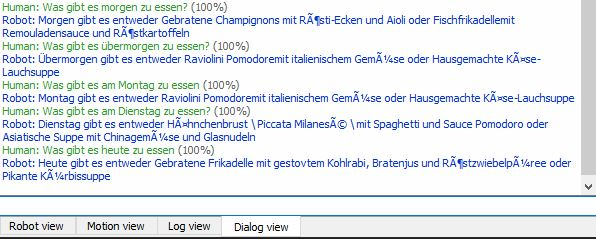
\includegraphics[width=\textwidth]{Figures/AppChapter/mensa_6.JPG}
    \caption{Mensa Dialog}
    \label{fig:mensadialog}
    \centering
\end{figure}


\section{Stundenplan}

Der zweite Anwendungsfall ist das Anzeigen des Stundenplans für jeden Studiengang und für jedes Semester. 
\\\\
…
\\
\subsection{Anzeigen des Stundenplans in Android Studio}

Nachdem die Stundenplandaten im Server bereitgestellt wurden, war der nächste Schritt das Anzeigen des Stundenplans in Android Studio. 
Hierfür wurde ein neues Gesprächsthema in dem Haupt-Topic erstellt.

\begin{lstlisting}
u:({so} zeig{e} {er} {mir} {den} Stundenplan {fuer} {den} Studiengang 
_~Studiengaenge {[im "fuer das"]} semester _~semester {sofort} {bitte})

$course=$1 $semester=$2 Alles klar ^execute(VariableExecutor, 
timetable_course_semester, $course, $semester)
\end{lstlisting}

Damit der User den Stundenplan einsehen kann, erwartet Pepper zwei Wörter. Der User muss in seiner Frage den Studiengang und das Semester 
nennen. Erst dann wird der Methodenaufruf gestartet. Somit werden die drei Parameter ``timetable\_course\_semester'', 
``\$course'' und ``\$semester'' mitgegeben.

\begin{lstlisting}
final String timetableurl = "https://informatik.hs-bremerhaven.de/
    docker-hbv-kms-http/api/v1/timetable?course="
    + course_ + "&semester="
    + semester_ + "&htmlOnly=true";

ma.runOnUiThread(() -> {
	ma.setContentView(R.layout.webtest);

	WebView web = (WebView) ma.findViewById(R.id.webView);
	WebSettings webSettings = web.getSettings();
	webSettings.setJavaScriptEnabled(true);
	web.setWebViewClient(new Callback());
	web.loadUrl(url);
});
\end{lstlisting}

Auf dem Node Server erwartet die API, die wir für den Stundenplan erstellt haben, bestimmte Parameter zu dem Studiengang und dem Semester. 
Hierfür können wir unsere Parameter, die in der Frage ermittelt wurden, in die Variable ``timetableurl'' einsetzen und erhalten 
die URL zu dem richtigen Stundenplan. Dieser kann anschließend mithilfe des Webviewers auf dem Tablet von Pepper angezeigt werden. 

\section{Routenfinder}

Der dritte und letzte Anwendungsfall ist die Navigationshilfe in der Hochschule Bremerhaven. Sollte der User einen bestimmten Raum oder ein 
Gebäude suchen, soll Pepper auf seinem Tablet eine genaue Wegbeschreibung geben können. 
\\\\
...
\\
\textbf{Videos in /var/www/hbv-kms abgelegt}
\\


\subsection{Anzeigen des Gebäudeplans und des Raumfinders in Android Studio}

Da wir die einzelnen Videodateien auf dem Hopper abgelegt haben, brauchen wir für diesen Anwendungsfall die Kommunikation mit dem Node Server nicht. 
Die JSON Datei, die mit dem Python Script erzeugt wurde, haben wir in den Assets Ordner in Android Studio abgelegt, um sie später im Code verwenden zu können. 

Wie bei allen anderen Anwendungsfällen auch, ist der erste Schritt das Erstellen der einzelnen Gesprächsthemen. 
Zuerst werden wir den Fall abdecken, wenn sich der User den Gebäudeplan anzeigen lassen will.

\begin{lstlisting}
u:([zeig gib] {mir} {bitte} {den} [Gebaeudeplan Campusplan Gelaende])
^execute(VariableExecutor, qiVariableNav, Plan) Hier hast du eine 
    Uebersicht ueber das Hochschulgelaende
\end{lstlisting}


\begin{lstlisting}
String nav = params.get(1);
if(nav.equals("Plan")) {
    try {
        ma.runOnUiThread(() -> {
            ma.setContentView(R.layout.campus_plan);
        });
    } catch (Exception e) {
        e.printStackTrace();
    }
}
\end{lstlisting}

\ref{fig:gplan} Sobald der User nach dem Gebäudeplan fragt, wird ein vordefiniertes XML-Layout mit einem Bild von dem 
Gebäudeplan auf dem Tablet angezeigt. Das Bild wurde vorher heruntergeladen und in den Ordner 
``drawable'' gelegt.

\begin{figure}[H]
    \centering
    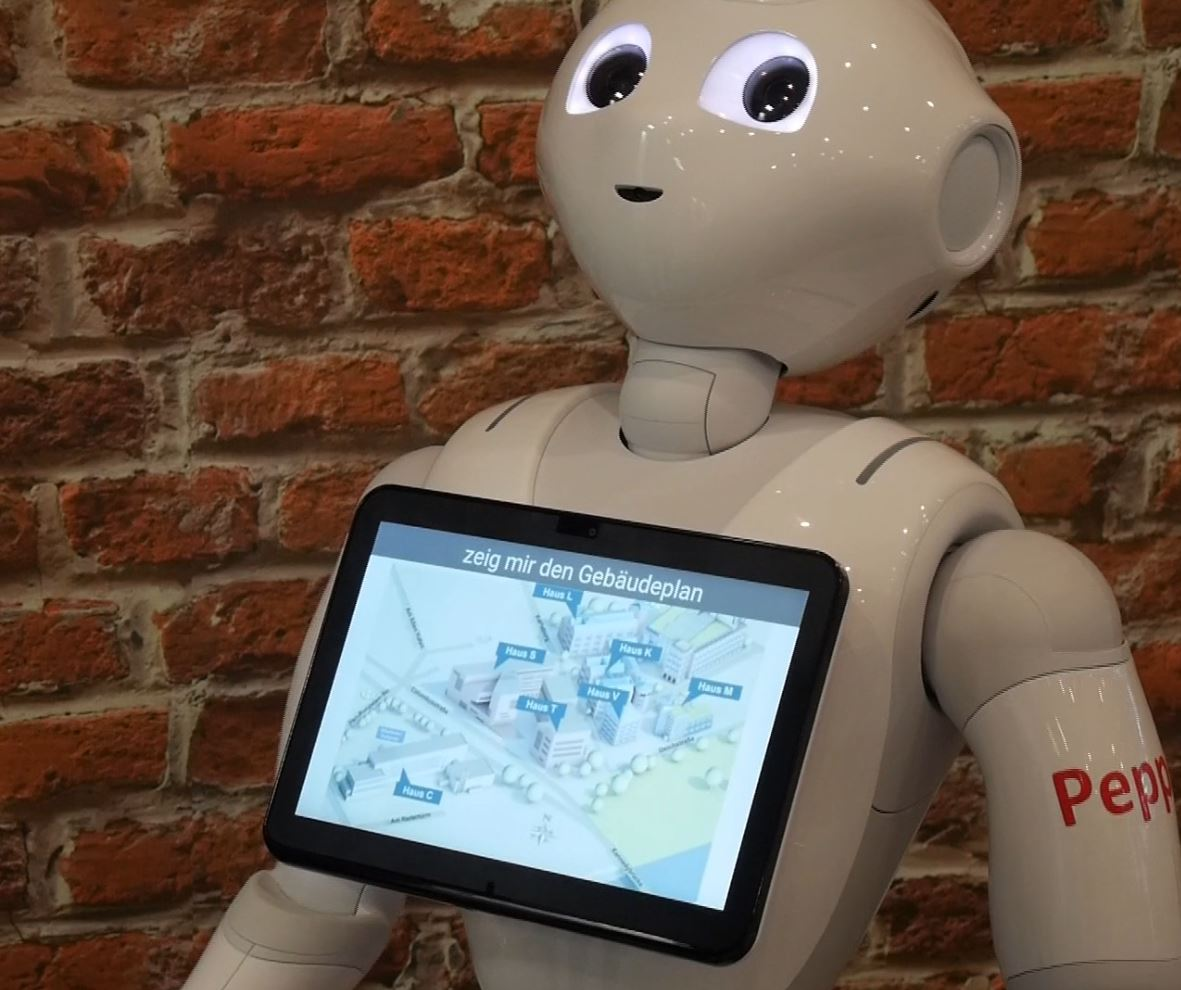
\includegraphics[width=10cm]{Figures/AppChapter/rx3.JPG}
    \caption{Gebäudeplan - Pepper}
    \label{fig:gplan}
    \centering
\end{figure}

Als Nächstes haben wir das Abrufen der Videodateien zu den einzelnen Räumen der Hochschule in Android 
Studio implementiert.

\begin{lstlisting}
concept:(rooms) [C006 C007 ... Z5150 Z5160 ]

u:(["{Kannst du {mir} [sagen erzaehlen]} Wo [befindet ist] {sich} der 
Raum _~rooms {befindet}"])
    $room=$1 Sofort ^execute(VariableExecutor, qiVariableNav, $room)
\end{lstlisting}

Pepper muss in der Lage sein, alle Räume in der Hochschule zu kennen, um genau herausfiltern zu können, welchen Raum der User sucht.
Das Konzept ``rooms'' beinhaltet alle Räume der Hochschule und wird somit in der Frage im Topic verwendet. Sollte der User 
nach einen Raum fragen, den es nicht gibt, wird Pepper die Frage erst gar nicht verstehen und nicht antworten. 

Sollte Pepper den Raum kennen, wird ein Methodenaufruf mit den Parametern ``qiVariableNav'' und der Raumnummer 
(``\$room'') durchgeführt.

\begin{lstlisting}
u:(Zeig mir {bitte} einen _~handicapped Weg [zu in] {dem} 
Raum _~rooms)
    $handicap=$1 $room=$2 Alles klar ^execute(VariableExecutor, 
    qiVariableNav, $room, $handicap)
\end{lstlisting}

Wenn der User explizit nach einem barrierefreien Weg zu einem Raum fragt, wird der gleiche Methodenaufruf mit dem zusätzlichen 
Parameter ``\$handicap'' durchgeführt.

\begin{lstlisting}
String room = nav;
String handicapped = "M0000";
if(params.size() == 3) handicapped = "M0001";
\end{lstlisting}


In der VariableExecutor Klasse wird als Erstes überprüft, ob der User nach einem barrierefreien Weg zu dem gewünschten Raum 
gefragt hat oder nicht. Mit einer If-Bedingung wird die Länge der Parameter überprüft, die in der Methode mitgegeben wurde. 
Wie bereits erwähnt, wird ein zusätzlicher Parameter ``\$handicap'' zusammen mit den Parametern ``qiVariableNav'' 
und ``\$room'' mitgegeben, wenn nach dem barrierefreien Weg gefragt wurde. Somit muss nur die Parameterlänge verglichen 
werden, um entscheiden zu können, welcher Weg angezeigt werden soll.

\begin{lstlisting}
BufferedReader reader = new BufferedReader(new InputStreamReader(
    ma.getAssets().open("route_metadata.json")));

String response = new String();
for (String line; (line=reader.readLine())!=null; response+=line);

Map jsonJavaRootObject = new Gson().fromJson(response, Map.class);

String path = ((Map)((Map)(jsonJavaRootObject.get(room)))
    .get(handicapped)).get("video_path").toString();
\end{lstlisting}

Mit der ``getAssets().open("route\_metadata.json")'' Funktion, kann die JSON Datei, die sich in dem ``assets'' 
Ordner befindet, geöffnet und mit dem BufferedReader ausgelesen werden. Als Nächstes wird mithilfe des Gson Frameworks, 
ein Map Objekt erzeugt, dass alle Informationen der JSON Datei bereitstellt. In der Variable ``path'', wird der Wert 
``video\_path'' mithilfe der genauen Raumnummer herausgesucht. Hier wird auch die Abfrage mitgegeben, ob der Weg 
Barrierefrei sein soll oder nicht.


\begin{lstlisting}
String urlVideo ="https://informatik.hs-bremerhaven.de/hbv-kms/"+path;
try{
    ma.runOnUiThread(() -> {
        ma.setContentView(R.layout.webtest);
        WebView web = (WebView) ma.findViewById(R.id.webView);
        WebSettings webSettings = web.getSettings();
        webSettings.setJavaScriptEnabled(true);
        web.setWebViewClient(new Callback());
        web.loadUrl(urlVideo);
    });
}
\end{lstlisting}

\ref{fig:Routenfinder} Nachdem der genau Pfad zum Video ermittelt wurde, kann nun die URL zu dem Video erstellt und mit dem Webviewer angezeigt werden.

\begin{figure}[H]
    \centering
    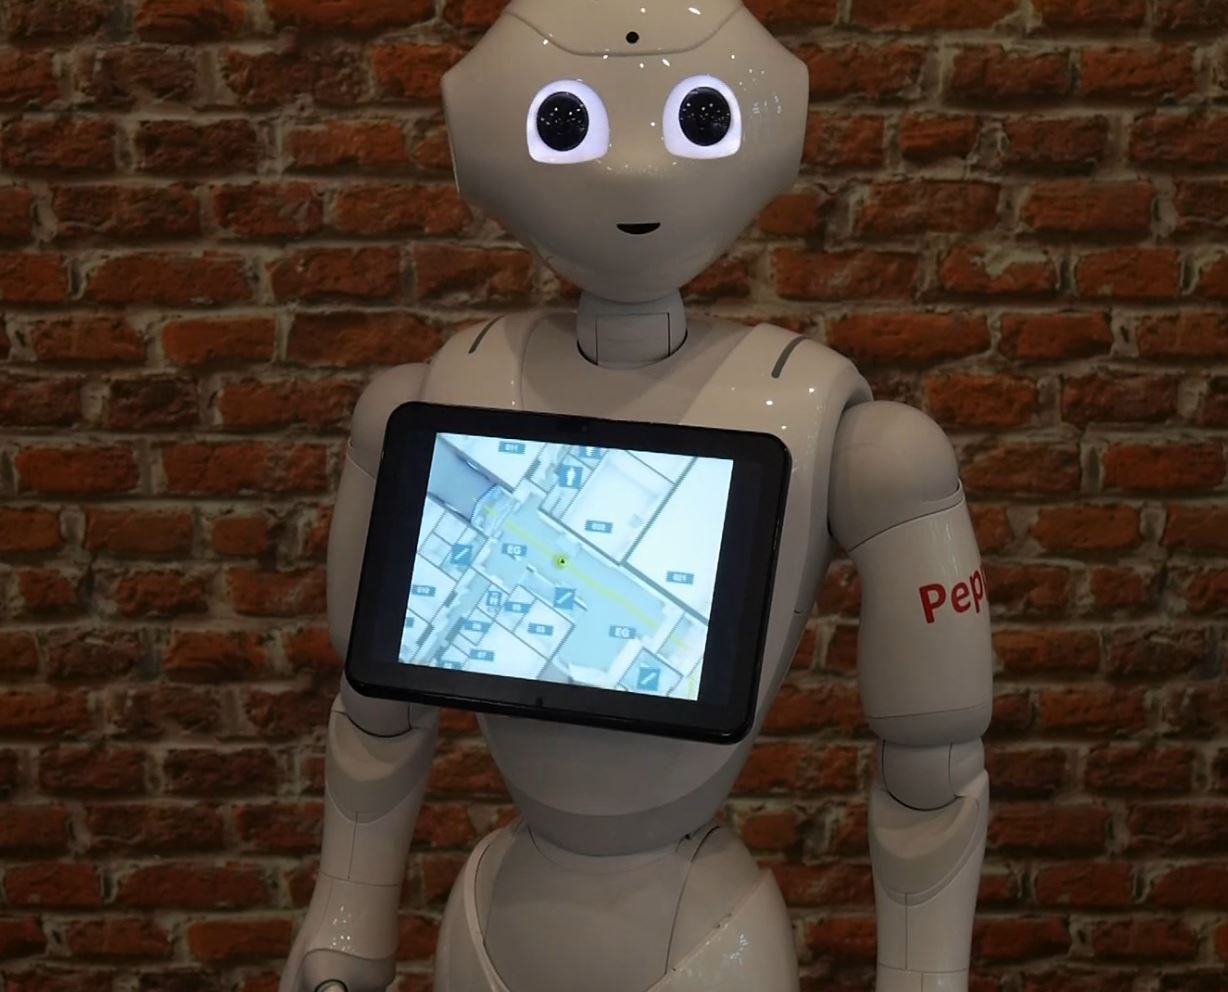
\includegraphics[width=10cm]{Figures/AppChapter/rx4.JPG}
    \caption{Routenfinder}
    \label{fig:Routenfinder}
    \centering
\end{figure}

\ref{fig:RoutenfinderDia} Zusätzlich zu dem Video soll Pepper dem User mit zusätzlichen Details antworten. Er gibt an, in welchem Gebäude sich der gesuchte Raum befindet, 
wie weit dieser von seinem Standpunkt entfernt ist und wie viel Zeit benötigt wird, um diesen Raum zu erreichen.

\begin{figure}[H]
    \centering
    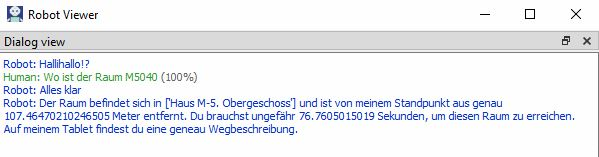
\includegraphics[width=\textwidth]{Figures/AppChapter/raumfinder_1.JPG}
    \caption{Routenfinder Dialog}
    \label{fig:RoutenfinderDia}
    \centering
\end{figure}


